Seperti yang telah dijelaskan pada \ref{sec:alternatif-solusi}, solusi yang dipilih adalah dengan mengkombinasikan antara sistem \textit{in-memory key-value store} milik Memcache dan menggunakan \textit{database} terpisah sebagai tempat penyimpanan data \textit{persistence}. Replikasi dan \textit{erasure coding} dapat dilakukan pada data persisten yang disimpan pada \textit{database} tersebut. Adapun gambaran umum arsitektur sistem dapat dilihat pada gambar \ref{fig:general-architecture}

\begin{figure}[ht]
    \centering
    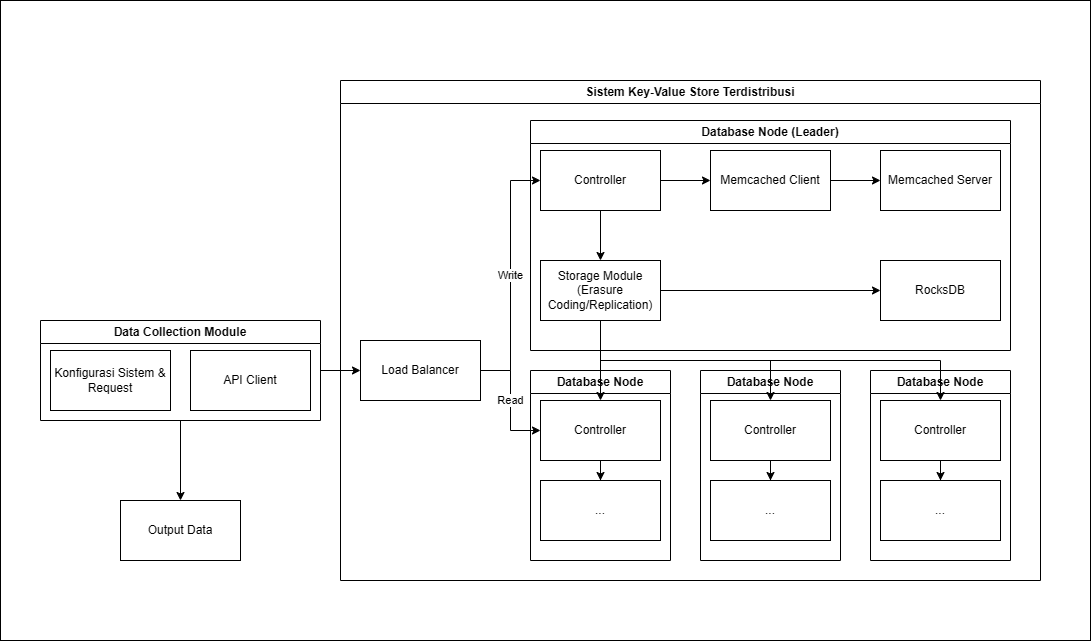
\includegraphics[width=0.95\textwidth]{resources/chapter-3/general-architecture.png}
    \caption{Gambaran Umum Arsitektur Sistem Eksperimen}
    \label{fig:general-architecture}
  \end{figure}